% Options for packages loaded elsewhere
\PassOptionsToPackage{unicode}{hyperref}
\PassOptionsToPackage{hyphens}{url}
%
\documentclass[
]{book}
\usepackage{amsmath,amssymb}
\usepackage{lmodern}
\usepackage{ifxetex,ifluatex}
\ifnum 0\ifxetex 1\fi\ifluatex 1\fi=0 % if pdftex
  \usepackage[T1]{fontenc}
  \usepackage[utf8]{inputenc}
  \usepackage{textcomp} % provide euro and other symbols
\else % if luatex or xetex
  \usepackage{unicode-math}
  \defaultfontfeatures{Scale=MatchLowercase}
  \defaultfontfeatures[\rmfamily]{Ligatures=TeX,Scale=1}
\fi
% Use upquote if available, for straight quotes in verbatim environments
\IfFileExists{upquote.sty}{\usepackage{upquote}}{}
\IfFileExists{microtype.sty}{% use microtype if available
  \usepackage[]{microtype}
  \UseMicrotypeSet[protrusion]{basicmath} % disable protrusion for tt fonts
}{}
\makeatletter
\@ifundefined{KOMAClassName}{% if non-KOMA class
  \IfFileExists{parskip.sty}{%
    \usepackage{parskip}
  }{% else
    \setlength{\parindent}{0pt}
    \setlength{\parskip}{6pt plus 2pt minus 1pt}}
}{% if KOMA class
  \KOMAoptions{parskip=half}}
\makeatother
\usepackage{xcolor}
\IfFileExists{xurl.sty}{\usepackage{xurl}}{} % add URL line breaks if available
\IfFileExists{bookmark.sty}{\usepackage{bookmark}}{\usepackage{hyperref}}
\hypersetup{
  pdftitle={Introduction à l'économie},
  pdfauthor={Dieye Abdoulaye},
  hidelinks,
  pdfcreator={LaTeX via pandoc}}
\urlstyle{same} % disable monospaced font for URLs
\usepackage{longtable,booktabs,array}
\usepackage{calc} % for calculating minipage widths
% Correct order of tables after \paragraph or \subparagraph
\usepackage{etoolbox}
\makeatletter
\patchcmd\longtable{\par}{\if@noskipsec\mbox{}\fi\par}{}{}
\makeatother
% Allow footnotes in longtable head/foot
\IfFileExists{footnotehyper.sty}{\usepackage{footnotehyper}}{\usepackage{footnote}}
\makesavenoteenv{longtable}
\usepackage{graphicx}
\makeatletter
\def\maxwidth{\ifdim\Gin@nat@width>\linewidth\linewidth\else\Gin@nat@width\fi}
\def\maxheight{\ifdim\Gin@nat@height>\textheight\textheight\else\Gin@nat@height\fi}
\makeatother
% Scale images if necessary, so that they will not overflow the page
% margins by default, and it is still possible to overwrite the defaults
% using explicit options in \includegraphics[width, height, ...]{}
\setkeys{Gin}{width=\maxwidth,height=\maxheight,keepaspectratio}
% Set default figure placement to htbp
\makeatletter
\def\fps@figure{htbp}
\makeatother
\setlength{\emergencystretch}{3em} % prevent overfull lines
\providecommand{\tightlist}{%
  \setlength{\itemsep}{0pt}\setlength{\parskip}{0pt}}
\setcounter{secnumdepth}{5}
\usepackage{booktabs}
\ifluatex
  \usepackage{selnolig}  % disable illegal ligatures
\fi
\usepackage[]{natbib}
\bibliographystyle{apalike}

\title{Introduction à l'économie}
\author{Dieye Abdoulaye}
\date{2021-07-22}

\begin{document}
\maketitle

{
\setcounter{tocdepth}{1}
\tableofcontents
}
\hypertarget{avant-propos}{%
\chapter*{Avant-Propos}\label{avant-propos}}
\addcontentsline{toc}{chapter}{Avant-Propos}

Ce syllabus est essentiellement destiné à des étudiants de l'enseignement
supérieur, en particulier des sections de bachelier des domaines économique, politique et social (classification ARES). Il est le fruit de nombreuses années d'enseignement de cette matière.

Le cours comporte 9 leçons. Au début de chacune d'entre elles sont fixés les objectifs. Le syllabus se veut très complet, illustré par des graphiques et des exemples tirés de l'histoire ou de l'actualité. Des tableaux chiffrés actualisés, des fiches de lecture et des articles permettent aux étudiants d'effectuer des travaux préparatoires. Le cours a été conçu pour qu'au-delà des principes de base incontournables, certaines thématiques présentées puissent être ou non développées durant l'exposé oral.

A la fin de chaque leçon figure un résumé reprenant les points clés. Ensuite viennent les exercices et applications : d'une part, un QCM permettant surtout d'affiner la précision du raisonnement de base et l'utilisation de la terminologique, d'autre part, des exercices et des questions de réflexion, classés selon leur niveau de difficultés.

L'étudiant peut également utiliser un manuel de référence.

Un des problèmes rencontrés par les étudiants est « comment étudier une
matière aussi volumineuse » ? Tout d'abord, il ne s'agit pas d'« étudier», mais bien d'acquérir un vocabulaire spécifique, des mécanismes de base et des outils d'analyse. De ce point de vue, \textcolor{red}{**l’assistance active au cours est primordiale**.}
Le support powerpoint utilisé est téléchargeable à l'issue de chaque leçon, ce qui permet à l'étudiant de revoir le cours chez lui. Il a donc reçu un syllabus complet, il a assisté au cours, il dispose des dias de l'exposé, d'un résumé et d'exercices, parmi lesquels les questions d'examen seront choisies (sauf QCM).

{\textbf{Schéma des leçons dans le syllabus}}

\begin{enumerate}
\def\labelenumi{\arabic{enumi}.}
\tightlist
\item
  Macro-objectif(s) tel(s) que défini(s) au dossier pédagogique de l'UE EPS.
\item
  Déclinaison du (des) macro-objectifs en compétences et plan de la leçon.
\item
  Matière : théories, exemples et explications, schémas, graphiques,..
\item
  Eventuellement : fiche(s) de lecture complémentaire(s), portefeuille de lectures.
\item
  Résumé (idées principales de la leçon).
\item
  QCM (avec réponses dans le syllabus, à la suite des exercices).
\item
  Exercices et questions de réflexion, notés selon le niveau de difficulté .
  Au terme de chaque leçon,
\end{enumerate}

\begin{itemize}
\tightlist
\item
  Powerpoint disponible sur l'intranet.
\item
  dans les 4 semaines, réponses aux questions disponibles sur l'intranet.
\end{itemize}

{\textbf{Portefeuille de lectures}}
Ces lectures font partie du cours ; elles éclairent les éléments théoriques et offrent des sujets de réflexion ; il est
donc indispensable de s'y attarder.

{\textbf{Comment « étudier » ?}}

\begin{itemize}
\tightlist
\item
  PAS de « par cœur » !!!
\item
  Lire systématiquement le cours, 1x, 2x, y compris les notes de bas de pages !
\item
  Assimiler les « NOTIONS A MAÎTRISER » indiquées au début des exercices (savoir de quoi on parle !)
\item
  Refaire les graphiques et les raisonnements, en travaillant avec le PP
\item
  Faire un maximum d'exercices, et s'auto-évaluer à l'aide des réponses
\item
  S'intéresser à l'actualité économique, visionner quelques sites internet renseignés.
\end{itemize}

\hypertarget{pruxe9sentation-globale}{%
\chapter*{Présentation Globale}\label{pruxe9sentation-globale}}
\addcontentsline{toc}{chapter}{Présentation Globale}

{\textbf{MACRO-OBJECTIFS }} (dossier pédagogique de l'UE)

\begin{enumerate}
\def\labelenumi{\arabic{enumi}.}
\tightlist
\item
  présenter et d'analyser de manière critique les principaux mécanismes économiques : le circuit
  économique fondamental et le rôle des différents facteurs et agents ;
\item
  analyser et confronter les fondements des principaux mouvements théoriques (classique, marxiste) en
  saisissant leurs relations avec les phénomènes politiques et sociaux.
\end{enumerate}

{\textbf{OBJECTIFS :}}
Au cours de cette leçon, l'étudiant va :

\begin{enumerate}
\def\labelenumi{\arabic{enumi}.}
\tightlist
\item
  se familiariser avec la notion de « science économique » ;
\item
  découvrir comment raisonnent les économistes, en distinguant les questions positives des questions normatives et en appréhendant la notion de modèle économique ;
\item
  analyser les deux lois fondamentales de l'économie : utilité marginale décroissante et rendements marginaux décroissants ;
\item
  appréhender la notion de frontière de possibilités de production (FPP) ;
\item
  expliciter des notions relatives aux deux courants théoriques fondateurs de la science économique :
  classicisme et marxisme ;
\item
  appréhender les problèmes économiques fondamentaux qui se posent à toute société et les
  systèmes d'allocation des ressources ;
\item
  analyser le rôle de l'Etat dans le système économique capitaliste.
\end{enumerate}

{\textbf{PLAN}}

Ce cours n'est évidemment pas exhaustif. Il ne couvre ni l'ensemble des théories ni l'entièreté du domaine économique. Après réflexion, nous avons aussi décidé d'organiser ce cours en trois chapitres.

\begin{itemize}
\item
  Le chapitre 1, intitulé \textcolor{red}{« Nature de l’activité économique et objet de la science économique »} en rappelle les définitions, les fondements et présente les principales méthodes et analyses économiques qui seront utilisées dans le reste de l'ouvrage.
\item
  Le chapitre 2, intitulé « Les grands courants de la pensée économique » éclaire cependant, à l'aide des théories et auteurs sur les principales écoles de la pensée économique contemporaine.
\item
  Le chapitre 3, intitulé « L'Economie et les autres sciences » examine les interactions et relations de l'économie avec les autres disciplines en
  particulier avec la Sociologie, la Géographie et l'environnement. Chacun peut être abordé indépendamment des autres, même si chacun s'appuie sur les résultats et analyses d'autres chapitres et y renvoie.
\end{itemize}

\hypertarget{intro}{%
\chapter{Introduction}\label{intro}}

En réalité, il n'existe pas une seule définition de l'économie, mais plusieurs définitions. Chaque définition renvoyant à des réalités sous-jacentes différentes. La définition de l'économie n'est pas consensuelle. Ses contours et son contenu varient en fonction des auteurs et des courants de pensée.

\hypertarget{nature-de-lactivituxe9-uxe9conomique-et-objet-de-la-science-uxe9conomique}{%
\chapter{Nature de l'activité économique et objet de la science économique}\label{nature-de-lactivituxe9-uxe9conomique-et-objet-de-la-science-uxe9conomique}}

Maitriser les définitions de l'économie, Connaître les méthodes
économiques et porter un éclairage sur les concepts de base de
l'économie sont les objectifs de ce chapitre premier.

\hypertarget{quest-ce-que-luxe9conomie}{%
\section{Qu'est-ce que l'économie?}\label{quest-ce-que-luxe9conomie}}

\hypertarget{besoins-illimituxe9s-et-biens-limituxe9s}{%
\section{Besoins illimités et biens limités}\label{besoins-illimituxe9s-et-biens-limituxe9s}}

\hypertarget{la-science-uxe9conomique-muxe9thodes-et-pruxe9occupations}{%
\section{La science économique: méthodes et préoccupations}\label{la-science-uxe9conomique-muxe9thodes-et-pruxe9occupations}}

\hypertarget{les-grands-courants-de-la-pensuxe9e-uxe9conomique}{%
\chapter{Les grands courants de la pensée économique}\label{les-grands-courants-de-la-pensuxe9e-uxe9conomique}}

\hypertarget{les-courants-fondateurs-de-la-pensuxe9e-uxe9conomique}{%
\section{Les courants fondateurs de la pensée économique}\label{les-courants-fondateurs-de-la-pensuxe9e-uxe9conomique}}

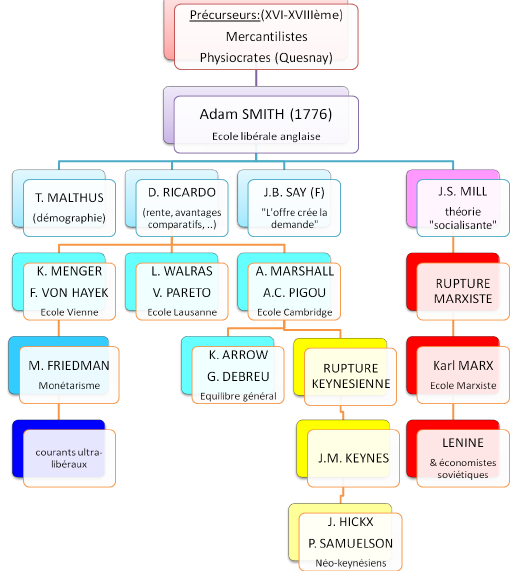
\includegraphics{_book/Book_files/figure-html/Syst_Eco.png}
\#\# La pensée contemporaine

\hypertarget{les-systuxe8mes-uxe9conomiques}{%
\section{Les systèmes économiques}\label{les-systuxe8mes-uxe9conomiques}}

\hypertarget{luxe9conomie-et-les-autres-sciences}{%
\chapter{L'économie et les autres sciences}\label{luxe9conomie-et-les-autres-sciences}}

\hypertarget{luxe9conomie-de-lenvironnement}{%
\section{l'économie de l'environnement}\label{luxe9conomie-de-lenvironnement}}

\hypertarget{leconomie-sociale}{%
\section{l'Economie sociale}\label{leconomie-sociale}}

\hypertarget{luxe9conomie-guxe9ographique}{%
\section{L'économie géographique}\label{luxe9conomie-guxe9ographique}}

You can write citations, too. For example, we are using the \textbf{bookdown} package \citep{CompuAct2014} in this sample book, which was built on top of R Markdown and \textbf{knitr} \citep{CompuAct2014}.

  \bibliography{book.bib,packages.bib}

\end{document}
